% -*- TeX-master: "main"; fill-column: 72 -*-

\section{Proposed syntax and semantics}
\label{sec:syntax}

In this section, we define the syntax and semantics of the Dynamic Structures package for SBML Level~3 Version~2. We delineate the data types and constructs defined in this package, then in \sec{sec:examples}, we provide complete examples of using the constructs in example SBML models.

\subsection{Overview of dyn extension}
\label{subsec:overview}

The primary mechanism this package uses to support dynamic cellular behavior are the \Event and \EventAssignment constructs. The Dynamic Structures package extends these components not only to allow modelers to indicate at which point during simulation (i.e., under what cellular conditions), but how certain SBML structural components (compartments or submodels) are affected in response to dynamic cellular processes. To fully enable this, dyn also extends the \Compartment object class to facilitate the representation of spatial rearrangements that follow dynamic cellular processes. Though such representations vary across tools based on the chosen modeling paradigm, this language extension defines the necessary constructs to enable tools to encode dynamic cellular behavior regardless of mathematical method or spatial representation framework.

{\color{red} Harold: \notice Out of the types of off-lattice frameworks, our proposed approach only covers center-based (objects spatially identified by the coordinates of their center of mass) and doesn't support vertix-based (where each object has several vertices that together uniquely describe its position)}

\subsection{Namespace URI and other declarations necessary for using this package}
\label{subsec:xml-namespace}

Every SBML Level~3 package is identified uniquely by an XML namespace URI.
For an SBML document to be able to use a given SBML Level~3 package, it
must declare the use of that package by referencing its URI.  The following
is the namespace URI for this version of the Dynamic Structures
package for SBML Level~3 Version~2:

\begin{center}
\uri{http://www.sbml.org/sbml/level3/version2/dyn/version1}
\end{center}

In addition, SBML documents using a given package must indicate whether
understanding the package is required for complete mathematical
interpretation of a model, or whether the package is optional.  This is
done using the attribute \token{required} on the \token{<sbml>} element in
the SBML document.  For the Dynamic Structure package, the value of
this attribute must be set to \val{true}.
The following fragment illustrates the beginning of a typical SBML model
using \sbmlthreecore and this version of the dyn package:

\begin{example}
<?xml version="1.0" encoding="UTF-8"?>
<sbml xmlns="http://www.sbml.org/sbml/level3/version2/core" level="3" version="2"
      xmlns:fbc="http://www.sbml.org/sbml/level3/version2/dyn/version1" arrays:required="true">
\end{example}

\subsection{Primitive data types}
\label{subsec:primitives}
The Dynamic Structure package uses a number of the primitive data types described in Section 3.1 of the \sbmlthreecore specification as well as a number of XML Schema 1.0 data types~\citep{biron:2000}. More specifically, we make use of \primtype{SId}, \primtype{int}, and \primtype{SIdRef}. This package also adds additional primitive data types described below.

\subsubsection{\emph{Type} \primtype{CBOTerm}}
\label{dat:CBOTerm}

The type \primtype{CBOTerm} is used as the data type of the attribute \token{cboTerm} on the \Event object class. \primtype{CBOTerm} follows the syntax defined for the \primtype{anyURI} data type, which considers it a character string data type whose values are interpretable as URIs~(Universal Resource Identifiers; \citep{Means:2001}; \citep{w3c:2000b}) as described by the W3C document RFC 3986 \citep{Berners-Lee:2005}. Examples of valid string values of type CBOTerm are:  
\begin{center}
\url{http://cbo.biocomplexity.indiana.edu/svn/cbo/trunk/CBO_1_0.owl#Apoptosis} \url{http://cbo.biocomplexity.indiana.edu/svn/cbo/trunk/CBO_1_0.owl#Movement}
\end{center}
These values are meant to be the identifiers of terms from the Cell Behavior Ontology (CBO) whose curated vocabulary describes cellular entities and processes in computational models. \sec{sec:CBO} provides more information about the ontology, supported ontological terms and general principles for their use in SBML models.

\subsubsection{\emph{Type} \primtype{CoordinateSystemKind}}
\label{dat:CoordSystemKind}

Type \primtype{CoordinateSystemKind} is a primitive data type that is used in extending the \Compartment object to indicate the coordinate system in which the position of modeling elements is to be specified. \primtype{CoordinateSystemKind} is derived from the basic \primtype{XML} type \primtype{string}, but with restrictions about the sequences in which characters may appear. Values for attributes of this data type can only include: \val{cartesian}. The meaning of each of these values is discussed in the context of the extended \Compartment object in \sec{subsec:extCompartment}.

{\color{red} Harold: \notice  If we indicate a coordinateSystem such as cartesian, we should also support other such as "cylindrical", "spherical", and "polar" (which the spatial package also supports). It would make for a more 
	
If SED-ML is used, using more coordinate systems would mean that not only would we need to worry about translating how dynamic processes are represented across spatial frameworks, but coordinate systems! (Another layer of complexity)}

\subsubsection{\emph{Type} \primtype{CoordinateKind}}
\label{dat:CoordKind}

The \primtype{CoordinateKind} primitive data type is used in the definition of the \CoordinateComponent class. \primtype{CoordinateKind} is derived from the basic \primtype{XML} type \primtype{string} though it restricts possible values attributes of this data type can take. Supported values include: \val{cartesianX}, \val{cartesianY}, \val{cartesianZ}. Attributes of \primtype{CoordinateKind} type are discussed in the context of the extended \Compartment object in \sec{subsec:extCompartment}.

{\color{red} Harold: \notice If cylindrical, spherical and polar coordinate systems are used, the list of possible values for this data type would need to be extended to include: "sphericalRadius", "sphericalAzimuth", "sphericalElevation", "cylindrical-Radius", "cylindricalAzimuth", "cylindricalHeight", "polarRadius", and "polarAzimuth". }

\subsection{The extended \class{Event} object}
\label{subsec:extEvent}

The \Event class is extended in the Dynamic Structure package. The addition of a \token{cboTerm} attribute is designed to allow a modeler or a software package to attach semantical information to events triggered in response to dynamic cellular processes in an SBML model. \ref{fig:UMLExtendedEvent} provides the corresponding UML diagram. 

\begin{figure}[tbhp]
  \centering
  %\usepackage{graphicx}
  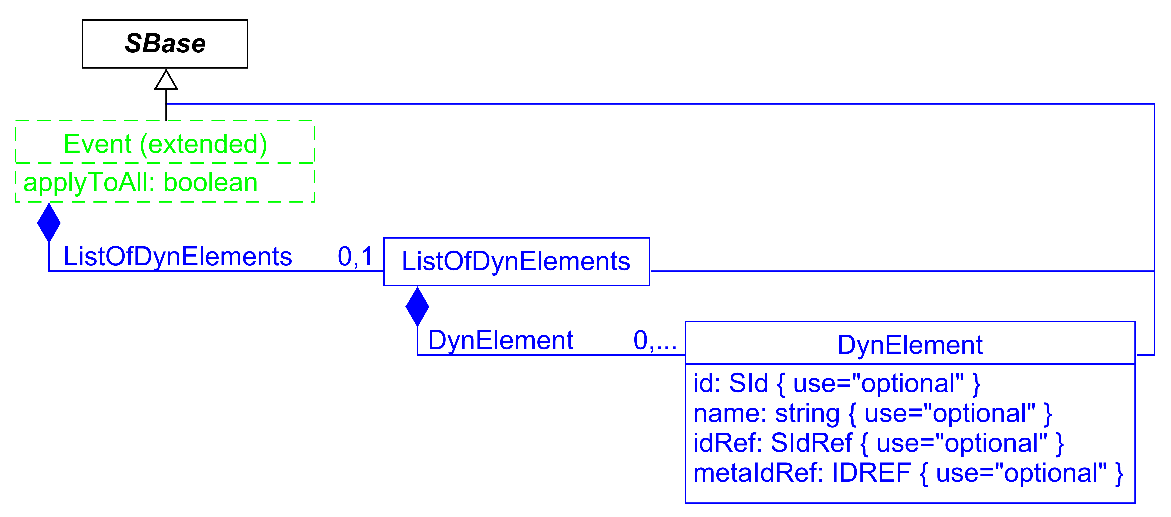
\includegraphics[width=0.25\textwidth]{images/UMLExtendedEvent.pdf}\\
  \caption{A UML representation of the extended \Event class. See \ref{subsec:conventions}} for conventions related to this figure. \label{fig:UMLExtendedEvent}
\end{figure}

\subsubsection{The \token{cboTerm} attribute}
\label{attr:cboTerm}

The attribute called \token{cboTerm} on the \Event class supports the use of Cell Behavior Ontology(CBO) terms to provide semantic encoding of dynamic cellular events in SBML models. By adding CBO terms, modelers can semantically annotate event constructs to explicitly indicate which cellular processes are being modeled in each \Event instance. The relationship is of the form "the Event is-a X", where X is the CBO term. The term chosen should be the most precise one that captures the role of the Event in the model. The value of \token{cboTerm} must conform to the syntax permitted by the \primtype{CBOTerm} data type previously described in \sec{dat:CBOTerm} of the current specification. The scope of the \token{cboTerm} attribute is local to the enclosing object definition and is not visible outside the object definition. For a discussion on supported values for \token{cboTerm} and CBO in general see \sec{sec:CBO}

\subsection{The extended \class{EventAssignment} object}
\label{subsec:extEventAssignment}

In every instance of an event definition in a model, the subobject \ListOfEventAssignments element must have a non-empty list of one or more elements of class \EventAssignment. This package extends the \EventAssignment class to add a \token{component} attribute to allow modelers to indicate which cellular structures are involved in an event executed to model dynamic cellular behavior. The definition for the extension of the \EventAssignment element is shown in \ref{fig:UMLExtendedEventAssignment}.
 
\begin{figure}[tbhp]
	\centering
	%\usepackage{graphicx}
	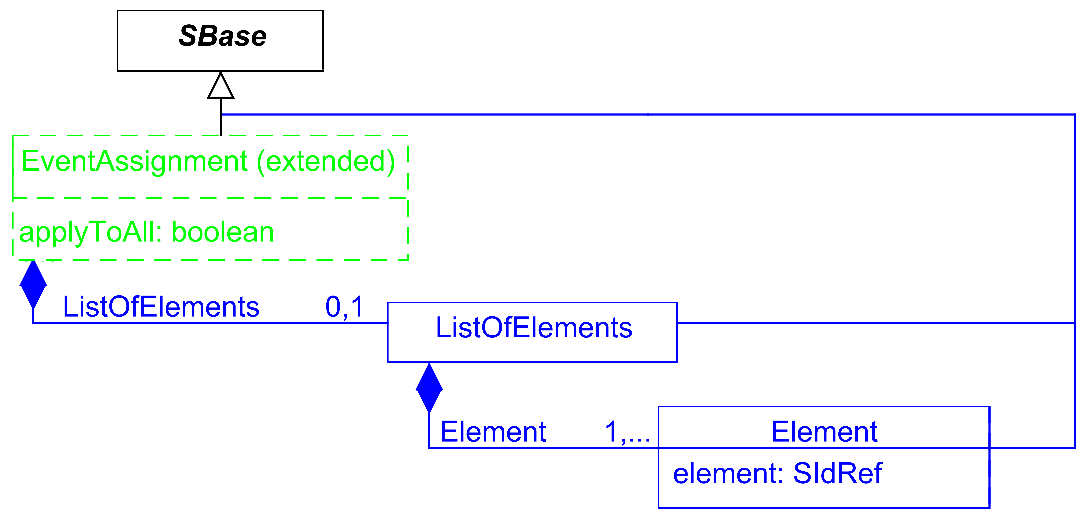
\includegraphics[width=0.25\textwidth]{images/UMLExtendedEventAssignment.pdf}\\
	\caption{A UML representation of the extended \EventAssignment class. See \ref{subsec:conventions}} for conventions related to this figure. \label{fig:UMLExtendedEventAssignment}
\end{figure}

\subsubsection{The \token{component} attribute}
\label{attr:component}

\token{Component} is a mandatory attribute of the type \primtype{SidRef} that is used to uniquely identify the cellular structure (either compartment or submodels) to be dynamically altered when a dynamic event is executed. When this attribute points to \Compartment elements, they must have a child \ListOfCoordinateComponents as seen in \ref{subsec:extCompartment}. This ensures that when an extended event is executed, referenced cellular compartments will have an assigned spatial location, which is necessary when modeling cellular behavior. If this is not the case, the \EventAssignment is not considered to be part of the dynamic representation of the model.

{\color{red} Harold: \notice How do we exactly indicate what happens to all the compartments within? Do we have separate EventAssignments-one for each contained element?}

\subsection{The extended \class{Compartment} object}
\label{subsec:extCompartment}

The \Compartment class must be extended to represent the spatial location and subsequent rearrangement that follows dynamic cellular processes emulated by extended \Event constructs. Refer to \sec{sec:CBO} for a list of supported dynamic cellular processes and associated ontological terms. This package adds the mandatory attribute \token{coordinateSystem} and subobjects \ListOfCoordinateComponents and \CoordinateComponent to describe the spatial location of modeling objects. \ref{fig:UMLExtendedCompartment} provides the corresponding UML diagram of the various features of the extended \Compartment class. 

{\color{red} Harold: \notice If we add a rotation attribute here to support 2D representations (bacterial growth) where rotation is important in spatially describing objects, how exactly do we do it? Rotation would be measured in what units (radians, degrees)? Would rotation be relative to a given coordinate component? 

Also, should the CoordinateSystem attribute reside in Compartment? If we only have one allowed value (cartesian) it doesn't matter. However, if we allow several possible coordinate systems (spherical,cylindrical, etc) users may indicate different ones for extended Compartments in the same model, which would be an error. As we cannot use defaults, I think this attribute should be more general so it applies to all Compartments at once.
}

\begin{figure}[tbhp]
	\centering
	%\usepackage{graphicx}
	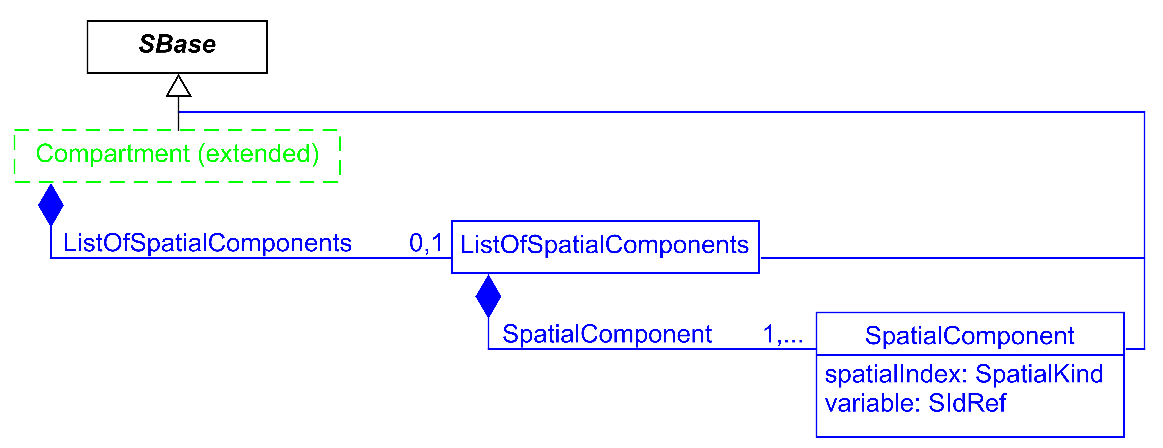
\includegraphics[width=0.85\textwidth]{images/UMLExtendedCompartment.pdf}\\
	\caption{UML diagram for the extension of the \Compartment object and the definition of \ListOfCoordinateComponents and \CoordinateComponent classes. See \ref{subsec:conventions} for conventions related to this figure.} \label{fig:UMLExtendedCompartment}
\end{figure}

\subsubsection{The \token{coordinateSystem} attribute}
\label{attr:coordSystem}

The \token{coordinateSystem} attribute is a required attribute of type \primtype{CoordinateSystemKind}. It represents the coordinate system used by a \Compartment to indicate its spatial location. A value of \val{cartesian} indicates that the \Compartment is in a cartesian coordinate system (1, 2 or 3D) and that the coordinate components correspond to the x, y, and z cartesian components.

%The CoordinateComponent class 3-dimensional). A value of “cylindrical” indicates that the geometry is a three-dimensional cylendrical coordinate system, with coordinate components corresponding to radial distance, azimuth angle, and axial position. A value of “spherical” indicates that the geometry is a three-dimensional spherical coordinate system, with coordinate components corresponding to radial distance, polar angle, and azimuth angle. A value of “polar” indicates that the geometry is a two-dimensional polar coordinate system, with coordinate components corresponding to radial distance and angle (the two-dimensional equivalent of the cylendrical coordinate system). 

{\color{red} Harold: \notice  Do we expect to model something of higher dimensions than 3D cartesian coordinate system? Specifying how the actual dynamic events are carried out in SED-ML is not only dependent on translating between spatial frameworks (off-lattice vs lattice-based), but on the dimension of the spaces indicated. We need to be careful!}

\subsubsection{The \class{ListOfCoordinateComponents} class}
\label{subsec:listCoordComp}

\Compartments mapped by an \EventAssignment construct must contain an element called listOfCoordinateComponents, of class \ListOfCoordinateComponents. This object contains a list of \CoordinateComponent objects that define the coordinate system in which the component is modeled. If mapped, a \Compartment cannot have an empty \ListOfCoordinateComponents list.

\subsection{The \class{CoordinateComponent} class}
\label{subsec:coordComp}

Instances of the \CoordinateComponent class represent individual coordinate components of the spatial location of mapped \Compartment structures that are involved in dynamic events. This construct defines two attributes: \token{coordinateIndex} and \token{variable}. Being derived from SBase, this class also has all the usual attributes and elements of its parent class.

{\color{red} Harold: \notice So far we've defined the coordinate system and components to each x,y,z triplet for all compartments involved but nowhere have we defined the minimum and maximum values of the coordinate axis along which objects are modeled.
}

\subsubsection{The \token{coordinateIndex} attribute}
\label{attr:coordIndex}

The attribute \token{coordinateIndex} of type \primtype{CoordinateKind} is added to uniquely identify a coordinate axes in the defined \token{coordinateSystem}. \token{CoordinateIndex} may take one of all the possible \primtype{CoordinateKind} values specified in \sec{dat:CoordKind}. A single \val{cartesianX} \CoordinateComponent can be used to define one-dimensional systems; two-dimensional systems are in turn characterized by having two \CoordinateComponent children with \token{coordinateIndex} values of \val{cartesianX} and \val{cartesianY}; and three-dimensional ones can be defined by having three \CoordinateComponent elements with \token{coordinateIndex} values of \val{cartesianX}, \val{cartesianY}, and \val{cartesianZ}. 

\subsubsection{The \token{variable} attribute}
\label{attr:variable}

The \token{variable} attribute of type \primtype{SidRef} contains the identifier of a \Parameter defined in the model to explicitly specify an object's position. The scope of the referenced \Parameter component must be global to the whole model and its \token{constant} attribute must be set to \val{false} as spatial location of the associated \Compartment may change in response to dynamic processes.

